%% ===========================================================================
%%  GRAPHICAL ABSTRACT -- standalone, submitted as a separate file.
%%  Build:  pdflatex graphical_abstract
%%  Raster: pdftoppm -png -r 150 graphical_abstract.pdf graphical_abstract
%% ===========================================================================
\documentclass[border=6pt]{standalone}
\usepackage{lmodern}
\usepackage[T1]{fontenc}
\usepackage[utf8]{inputenc}
\usepackage{amsmath}
\usepackage{xcolor}
\usepackage{tikz}
\usetikzlibrary{arrows.meta, positioning, calc, fit, backgrounds}

\definecolor{headerblue}{HTML}{1B4F72}
\definecolor{rulegray}{HTML}{9AA5B1}
\definecolor{perf5}{HTML}{1E8449}
\definecolor{perf1}{HTML}{E74C3C}
\definecolor{catbovw}{HTML}{C2185B}
\definecolor{catclip}{HTML}{1E8449}
\definecolor{phase1color}{HTML}{2980B9}
\definecolor{phase2color}{HTML}{1E8449}
\definecolor{phase3color}{HTML}{7D3C98}
\definecolor{phase4color}{HTML}{E67E22}

\begin{document}
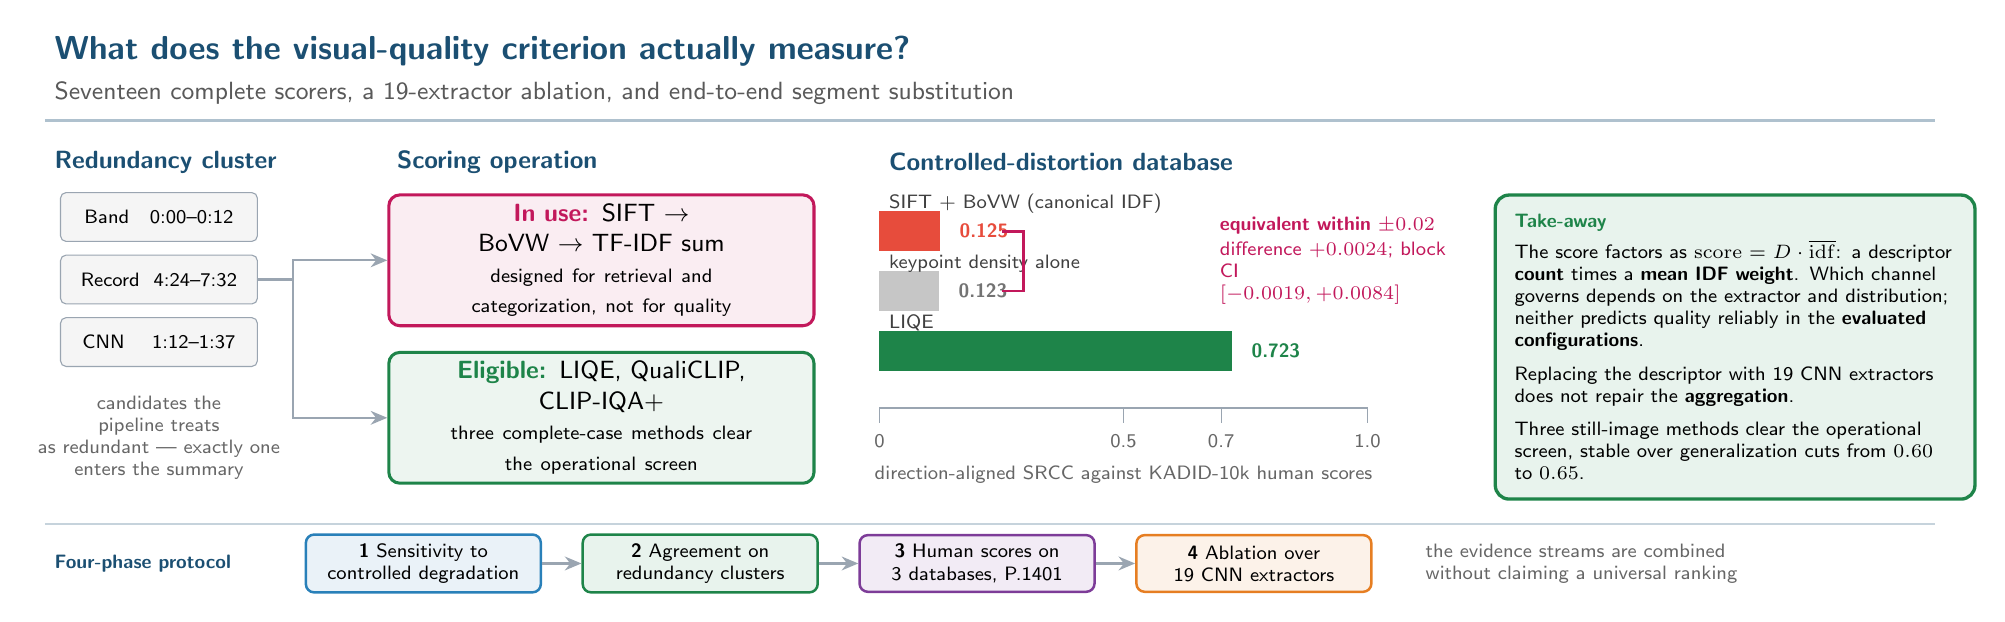
\begin{tikzpicture}[
  font=\sffamily,
  seg/.style={rectangle, rounded corners=2pt, minimum width=2.5cm,
    minimum height=0.62cm, draw=rulegray, fill=gray!8, font=\sffamily\scriptsize,
    align=center},
  segsel/.style={seg, draw=perf5, fill=perf5!14, font=\sffamily\scriptsize\bfseries},
  opbox/.style={rectangle, rounded corners=4pt, minimum width=5.4cm,
    minimum height=1.5cm, text width=5.1cm, align=center,
    font=\sffamily\small, line width=1.1pt},
  chip/.style={rectangle, rounded corners=3pt, minimum height=0.72cm,
    text width=2.75cm, align=center, font=\sffamily\scriptsize,
    line width=0.9pt},
  ar/.style={-{Stealth[length=6pt, width=5pt]}, thick, rulegray},
  ttl/.style={font=\sffamily\bfseries\small, text=headerblue},
]

%% ---------- Title strip ----------------------------------------------------
\node[font=\sffamily\bfseries\large, text=headerblue, anchor=west]
  at (0,5.15) {What does the visual-quality criterion actually measure?};
\node[font=\sffamily\small, text=black!65, anchor=west]
  at (0,4.62) {Seventeen complete scorers, a 19-extractor ablation, and
               end-to-end segment substitution};
\draw[headerblue!35, line width=1pt] (0,4.28) -- (24,4.28);

%% ---------- Stage 1: the input --------------------------------------------
\node[ttl, anchor=west] at (0,3.75) {Redundancy cluster};
\node[seg]    (sg1) at (1.45,3.05) {Band \ \ 0:00--0:12};
\node[seg, below=0.16cm of sg1] (sg2) {Record \ 4:24--7:32};
\node[seg, below=0.16cm of sg2] (sg3) {CNN \ \ \ 1:12--1:37};
\node[font=\sffamily\scriptsize, text=black!60, text width=3.1cm, align=center,
      below=0.24cm of sg3]
  {candidates the pipeline treats\\as redundant --- exactly one\\enters the summary};

%% ---------- Stage 2: the two operations ------------------------------------
\node[ttl, anchor=west] at (4.35,3.75) {Scoring operation};

\node[opbox, draw=catbovw, fill=catbovw!8, anchor=north west] (opA) at (4.35,3.35) {%
  \textcolor{catbovw}{\textbf{In use:}} SIFT $\rightarrow$ BoVW $\rightarrow$
  TF-IDF sum\\[3pt]
  {\scriptsize designed for retrieval and\\categorization, not for quality}};

\node[opbox, draw=catclip, fill=catclip!8, anchor=north west] (opB) at (4.35,1.35) {%
  \textcolor{catclip}{\textbf{Eligible:}} LIQE, QualiCLIP,\\CLIP-IQA$+$\\[3pt]
  {\scriptsize three complete-case methods clear\\the operational screen}};

\draw[ar] (sg2.east) -- ++(0.45,0) |- (opA.west);
\draw[ar] (sg2.east) -- ++(0.45,0) |- (opB.west);

%% ---------- Stage 3: the measurement ---------------------------------------
\node[ttl, anchor=west] at (10.6,3.75) {Controlled-distortion database};

\def\bx{10.6}      % bar origin x
\def\bw{6.2}       % full-scale width for |SRCC| = 1.0

% axis
\draw[rulegray, line width=0.7pt] (\bx,0.62) -- ({\bx+\bw},0.62);
\foreach \v/\lab in {0/0, 0.5/0.5, 0.7/0.7, 1.0/1.0}
  {\draw[rulegray] ({\bx+\v*\bw},0.62) -- ({\bx+\v*\bw},0.44);
   \node[font=\sffamily\scriptsize, text=black!60] at ({\bx+\v*\bw},0.20) {\lab};}
\node[font=\sffamily\scriptsize, text=black!60] at ({\bx+0.5*\bw},-0.22)
  {direction-aligned SRCC against KADID-10k human scores};

% bars
\fill[perf1] (\bx,2.62) rectangle ({\bx+0.125*\bw},3.12);
\node[font=\sffamily\scriptsize\bfseries, text=perf1, anchor=west]
  at ({\bx+0.125*\bw+0.12},2.87) {0.125};
\node[font=\sffamily\scriptsize, anchor=west, text=black!75]
  at (\bx,3.22) {SIFT $+$ BoVW (canonical IDF)};

\fill[gray!45] (\bx,1.86) rectangle ({\bx+0.123*\bw},2.36);
\node[font=\sffamily\scriptsize\bfseries, text=black!55, anchor=west]
  at ({\bx+0.123*\bw+0.12},2.11) {0.123};
\node[font=\sffamily\scriptsize, anchor=west, text=black!75]
  at (\bx,2.46) {keypoint density alone};

\fill[perf5] (\bx,1.10) rectangle ({\bx+0.723*\bw},1.60);
\node[font=\sffamily\scriptsize\bfseries, text=perf5, anchor=west]
  at ({\bx+0.723*\bw+0.12},1.35) {0.723};
\node[font=\sffamily\scriptsize, anchor=west, text=black!75]
  at (\bx,1.70) {LIQE};

% the equality bracket between the two 0.447 bars
\draw[catbovw, line width=1pt]
  ({\bx+0.125*\bw+0.78},2.87) -- ({\bx+0.125*\bw+1.05},2.87)
  -- ({\bx+0.125*\bw+1.05},2.11) -- ({\bx+0.125*\bw+0.78},2.11);
\node[font=\sffamily\scriptsize\bfseries, text=catbovw, anchor=west,
      text width=3.1cm]
  at (14.8,2.49) {equivalent within $\pm0.02$\\[1pt]
  {\scriptsize\mdseries difference $+0.0024$; block CI\\$[-0.0019,+0.0084]$}};

%% ---------- Stage 4: the take-away -----------------------------------------
\node[rectangle, rounded corners=5pt, draw=perf5, fill=perf5!10, line width=1.2pt,
      text width=5.6cm, align=left, font=\sffamily\scriptsize, anchor=north west,
      inner sep=7pt] (take) at (18.4,3.35) {%
  \textcolor{perf5}{\textbf{Take-away}}\\[3pt]
  The score factors as
  $\mathrm{score} = D \cdot \overline{\mathrm{idf}}$: a descriptor
  \textbf{count} times a \textbf{mean IDF weight}. Which channel governs depends
  on the extractor and distribution; neither predicts quality reliably in the
  \textbf{evaluated configurations}.\\[4pt]
  Replacing the descriptor with 19 CNN extractors does not repair the
  \textbf{aggregation}.\\[4pt]
  Three still-image methods clear the operational screen, stable over
  generalization cuts from $0.60$ to $0.65$.};

%% ---------- Bottom strip: the four phases ----------------------------------
\draw[headerblue!25, line width=0.8pt] (0,-0.85) -- (24,-0.85);
\node[font=\sffamily\bfseries\scriptsize, text=headerblue, anchor=west]
  at (0,-1.35) {Four-phase protocol};
\node[chip, draw=phase1color, fill=phase1color!10, anchor=west]
  (c1) at (3.3,-1.35) {\textbf{1} Sensitivity to\\controlled degradation};
\node[chip, draw=phase2color, fill=phase2color!10, right=0.5cm of c1]
  (c2) {\textbf{2} Agreement on\\redundancy clusters};
\node[chip, draw=phase3color, fill=phase3color!10, right=0.5cm of c2]
  (c3) {\textbf{3} Human scores on\\3 databases, P.1401};
\node[chip, draw=phase4color, fill=phase4color!10, right=0.5cm of c3]
  (c4) {\textbf{4} Ablation over\\19 CNN extractors};
\draw[ar] (c1) -- (c2); \draw[ar] (c2) -- (c3); \draw[ar] (c3) -- (c4);
\node[font=\sffamily\scriptsize, text=black!60, anchor=west, right=0.55cm of c4,
      text width=4.4cm]
  {the evidence streams are combined without claiming a universal ranking};

\end{tikzpicture}
\end{document}
